\documentclass[11pt,a4paper]{article}
\usepackage[utf8]{inputenc}
\usepackage[T1]{fontenc}
\usepackage[spanish,es-noshorthands]{babel}
\usepackage{amsmath,amssymb,amsthm}
\usepackage{bm}
\usepackage{geometry}
\geometry{margin=2.5cm}
\usepackage{graphicx}
\graphicspath{{../figuras/}}
\usepackage{float}
\usepackage{xcolor}
\usepackage{hyperref}
\hypersetup{colorlinks=true,linkcolor=blue!50!black,citecolor=blue!50!black,urlcolor=blue!50!black}
\usepackage{enumitem}
\usepackage{booktabs}
\newtheorem{definition}{Definición}
\newtheorem{remark}{Observación}
\newcommand{\R}{\mathbb{R}}
\newcommand{\thetavec}{\bm{\theta}}
\newcommand{\transp}{^{\top}}
\newcommand{\promptIA}[1]{\begin{center}\fcolorbox{gray}{gray!8}{\parbox{0.9\linewidth}{\small\textbf{[FIGURA -- PROMPT IA]}\\[2pt]#1}}\end{center}}
\title{\textbf{El modelo de Wilson--Cowan}\\[2pt]\large B3 --- El sistema dinámico que genera nuestros datos}
\author{Proyecto Wilson--Cowan --- Iniciación a la I+D ITBA}
\date{\today}
\begin{document}
\maketitle
\tableofcontents
\bigskip

\begin{remark}
Este documento supone que ya viste \textbf{B2} (neuronas, sinapsis y actividad poblacional) y \textbf{M2} (EDOs y sistemas dinámicos: equilibrios, Jacobiano, nulclinas, ciclo límite y bifurcación de Hopf). Acá juntamos las dos cosas: mostramos cómo dos poblaciones de neuronas se escriben como un sistema de dos EDOs y por qué ese sistema, con los parámetros adecuados, \emph{oscila}. Es el ``sistema real'' que produce los datos sintéticos que después intentamos identificar (ver P4, neural\_ode).
\end{remark}

\section{Historia y motivación}

\subsection{El problema en 1972}
A comienzos de los 70 la neurociencia teórica tenía un modelo excelente para \emph{una} neurona: Hodgkin y Huxley (1952) habían descrito con ecuaciones de conductancias iónicas cómo se dispara un potencial de acción. El problema es que la corteza no tiene una neurona: tiene del orden de $10^5$ neuronas por milímetro cúbico, densamente interconectadas. Simular cada una con Hodgkin--Huxley era (y sigue siendo) intratable, y además no era claro que sirviera: lo que se mide con un electrodo extracelular, un EEG o hoy una señal de calcio no es el disparo de \emph{una} célula, sino la \textbf{actividad agregada} de una población.

Hugh Wilson y Jack Cowan se hicieron una pregunta distinta: en vez de seguir cada neurona, ¿podemos escribir una ecuación para la \emph{fracción de neuronas activas por unidad de tiempo} en una población? Esa cantidad --- la \textbf{tasa de disparo poblacional} (\emph{firing rate}) --- es justamente lo que un experimento poblacional observa. El paso conceptual es el de la mecánica estadística: renunciar al detalle microscópico (qué hace cada neurona) para quedarse con una variable macroscópica (cuánto dispara la población en promedio).

\subsection{La idea de las dos poblaciones}
La segunda decisión clave fue \emph{qué} poblaciones considerar. En la corteza las neuronas se dividen a grandes rasgos en dos clases funcionales:
\begin{itemize}[nosep]
    \item \textbf{Excitatorias (E)}: al disparar, empujan hacia arriba la actividad de sus blancos (típicamente neuronas piramidales, glutamatérgicas).
    \item \textbf{Inhibitorias (I)}: al disparar, frenan la actividad de sus blancos (interneuronas GABAérgicas).
\end{itemize}
Wilson y Cowan (1972) modelaron un ``parche'' de tejido como \textbf{dos poblaciones acopladas}, $E$ e $I$, que se influyen mutuamente y a sí mismas. La intuición biológica es que muchos fenómenos interesantes --- oscilaciones, biestabilidad, histéresis --- no salen de una sola población sino del \emph{tira y afloje} entre excitación e inhibición. Este tipo de descripción se conoce hoy como modelo de \emph{masa neuronal} (\emph{neural mass}) y es el abuelo de casi todos los modelos de dinámica poblacional cortical.

\begin{figure}[H]\centering
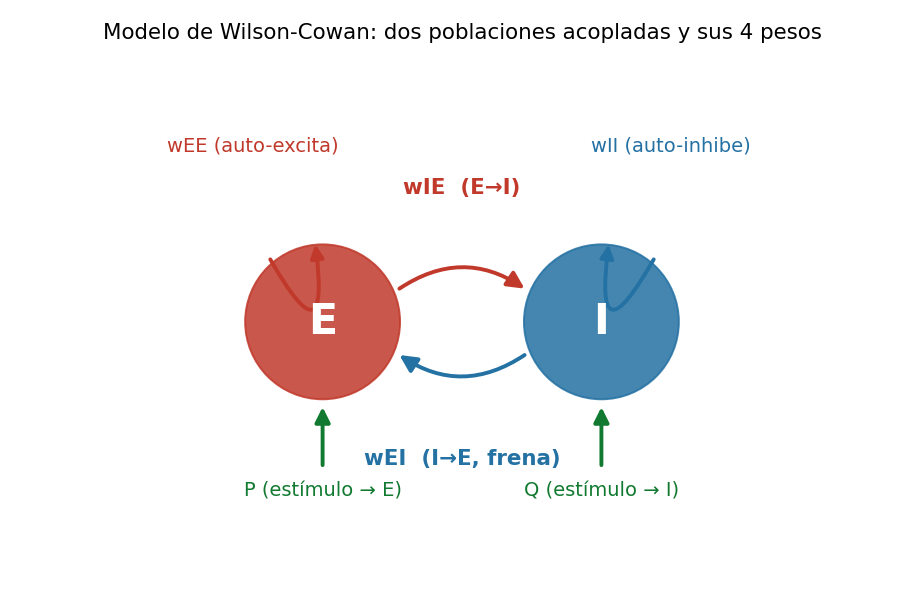
\includegraphics[width=0.75\linewidth]{fig_red_EI.png}
\caption{Esquema de la red de dos poblaciones. La población excitatoria $E$ y la inhibitoria $I$ se acoplan mediante cuatro pesos sinápticos ($w_{EE},w_{EI},w_{IE},w_{II}$) y reciben estímulos externos $P$ (a $E$) y $Q$ (a $I$). Es la estructura que las dos ecuaciones formalizan. (figura del proyecto)}
\label{fig:red}
\end{figure}

\section{Derivación de las dos ecuaciones}

\subsection{El ingrediente 1: relajación}
Pensemos primero en una sola población con actividad $E(t)$ (la fracción de neuronas activas). Si la dejamos sola, sin ninguna entrada, la actividad debería \emph{decaer} hacia el reposo: las neuronas que dispararon entran en refractario y dejan de contribuir. La forma más simple de escribir ese decaimiento es una relajación exponencial,
\[
\tau_e\,\dot E = -E,
\]
donde $\tau_e$ es la constante de tiempo: qué tan rápido la población ``olvida'' su actividad y vuelve al reposo. Cuanto mayor $\tau_e$, más lenta la población.

\subsection{El ingrediente 2: la entrada total pasada por una sigmoidea}
Ahora sumamos la entrada. Cada población recibe influencias de varias fuentes, y lo natural es sumarlas en una \textbf{entrada total} (o corriente sináptica neta). Para la excitatoria:
\[
u_e = \underbrace{w_{EE}\,E}_{\text{autoexcitación}} \;-\; \underbrace{w_{EI}\,I}_{\text{freno de I}} \;+\; \underbrace{P(t)}_{\text{estímulo externo}} \;-\; \underbrace{\theta_e}_{\text{umbral}}.
\]
Pero la actividad de la población \emph{no} es proporcional a $u_e$: es una función saturante. Con poca entrada casi nadie dispara; a partir de cierto umbral la fracción de activas crece rápido; y con mucha entrada satura (no puede haber más del 100\% de la población activa). Esa curva en forma de S es la \textbf{función de respuesta sigmoidea}
\[
S_a(u) = \frac{1}{1+e^{-a u}},
\]
donde $a$ es la ganancia (qué tan abrupta es la S). El umbral $\theta_e$ ya viene restado dentro de $u_e$: mueve la curva a izquierda o derecha.

\begin{figure}[H]\centering
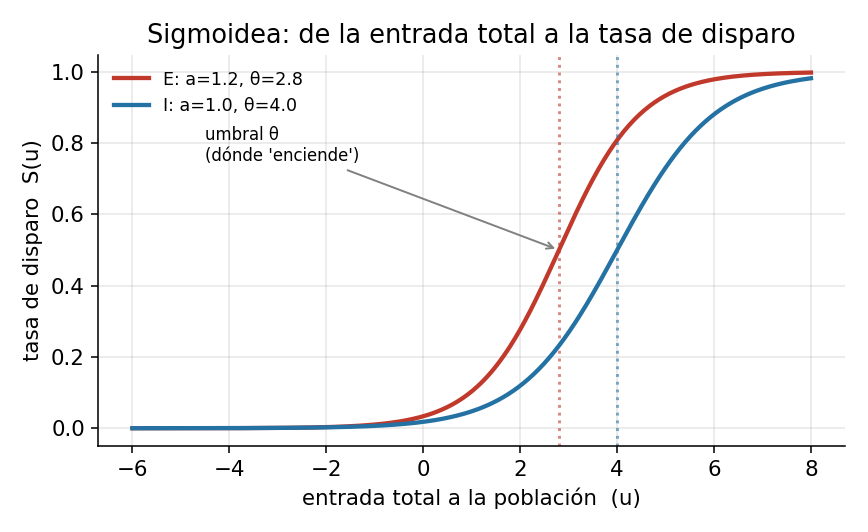
\includegraphics[width=0.7\linewidth]{fig_sigmoidea.png}
\caption{La función de respuesta sigmoidea $S_a(u)=1/(1+e^{-au})$ para las poblaciones $E$ e $I$. Convierte la entrada total $u$ de una población en su tasa de disparo, entre $0$ y $1$. La ganancia $a$ fija la pendiente y el umbral $\theta$ (ya restado en $u$) la desplaza horizontalmente. (figura del proyecto)}
\label{fig:sigmoidea}
\end{figure}

\subsection{Juntando todo}
Combinando relajación y entrada saturada, la población excitatoria evoluciona relajándose hacia el valor que le dicta su sigmoidea:
\[
\tau_e\,\dot E = -E + S_e\big(w_{EE}E - w_{EI}I + P(t) - \theta_e\big).
\]
Lo mismo para la inhibitoria, con sus propios pesos, umbral, ganancia y constante de tiempo, y con su estímulo $Q(t)$:
\[
\tau_i\,\dot I = -I + S_i\big(w_{IE}E - w_{II}I + Q(t) - \theta_i\big).
\]

\subsection{Fijar el reposo: los offsets $k_e,k_i$}
Hay un detalle importante. Sin estímulo ($P=Q=0$) nos gustaría que $E=I=0$ (poblaciones ``dormidas'' en reposo) sea un \emph{equilibrio}. Pero la sigmoidea no vale cero en el origen: $S_e(-\theta_e)=1/(1+e^{a_e\theta_e})>0$. Es decir, aún sin estímulo la sigmoidea empuja un poquito, y $E=0$ \emph{no} sería equilibrio. La solución es \textbf{restar ese valor de reposo}:
\[
k_e = \frac{1}{1+e^{a_e\theta_e}}, \qquad k_i = \frac{1}{1+e^{a_i\theta_i}}.
\]
Con esta corrección, en reposo el término de entrada se cancela exactamente y $\dot E=\dot I=0$. Escribiendo todo junto y dividiendo por las constantes de tiempo, quedan las \textbf{ecuaciones canónicas de Wilson--Cowan} que usamos en todo el proyecto. El estado es $\mathbf{x}=[I,E]$ (primero la inhibitoria, después la excitatoria, como en el código):
\begin{equation}
\boxed{\;
\begin{aligned}
\dot I &= \tfrac{1}{\tau_i}\big(-I + S_i(w_{IE}E - w_{II}I + Q(t) - \theta_i) - k_i\big),\\[4pt]
\dot E &= \tfrac{1}{\tau_e}\big(-E + S_e(w_{EE}E - w_{EI}I + P(t) - \theta_e) - k_e\big).
\end{aligned}
\;}
\end{equation}

\begin{remark}
Los offsets $k_e,k_i$ \textbf{no son parámetros libres}: se derivan de $(a_e,\theta_e)$ y $(a_i,\theta_i)$ respectivamente. En la identificación (ver P4) esto es clave: cuando cambiamos $\theta_e$ o $a_e$, recalculamos $k_e$ automáticamente para que el reposo siga siendo equilibrio, en vez de dejar que el optimizador ajuste un offset arbitrario que ``tape'' un mal ajuste de los umbrales.
\end{remark}

\section{Los diez parámetros y su significado biológico}

El modelo tiene exactamente \textbf{diez} parámetros. Identificarlos a partir de datos observados $y(t)$ es el objetivo central del proyecto. La Tabla~\ref{tab:params} lista los valores por defecto (los del simulador de MATLAB, ver §6) y qué significa cada uno.

\begin{table}[H]\centering
\begin{tabular}{@{}llcl@{}}
\toprule
Símbolo & Código & Valor & Qué es \\
\midrule
$w_{EE}$ & \texttt{wEE} & 6.4 & peso E$\to$E (autoexcitación) \\
$w_{EI}$ & \texttt{wEI} & 4.8 & peso I$\to$E (cuánto frena I a E) \\
$w_{IE}$ & \texttt{wIE} & 6.0 & peso E$\to$I (cuánto activa E a I) \\
$w_{II}$ & \texttt{wII} & 1.2 & peso I$\to$I (autoinhibición) --- \textbf{el difícil de identificar} \\
$\tau_e$ & \texttt{te} & 1.0 & constante de tiempo de E \\
$\tau_i$ & \texttt{ti} & 2.0 & constante de tiempo de I \\
$a_e$ & \texttt{ae} & 1.2 & ganancia sigmoidea de E \\
$a_i$ & \texttt{ai} & 1.0 & ganancia sigmoidea de I \\
$\theta_e$ & \texttt{thetae} & 2.8 & umbral sigmoidea de E \\
$\theta_i$ & \texttt{thetai} & 4.0 & umbral sigmoidea de I \\
\bottomrule
\end{tabular}
\caption{Los diez parámetros de Wilson--Cowan, con sus nombres en el código y los valores por defecto que reproducen el simulador MATLAB.}
\label{tab:params}
\end{table}

\paragraph{Los cuatro pesos sinápticos.} Cada $w$ dice \emph{cuánto} una población influye sobre otra (o sobre sí misma). Son adimensionales: multiplican tasas de disparo (entre 0 y 1) para producir corriente sináptica.
\begin{itemize}[nosep]
    \item $w_{EE}$: \textbf{autoexcitación} de E. Las piramidales se excitan entre sí; es el ``motor'' que puede disparar la actividad. Grande $\Rightarrow$ tendencia a explotar.
    \item $w_{EI}$: cuánto \textbf{frena} la inhibición a la excitación (I$\to$E). Es el freno principal que evita que E explote.
    \item $w_{IE}$: cuánto \textbf{activa} la excitación a la inhibición (E$\to$I). Cierra el lazo: si E sube, recluta a I, que a su vez frena a E. Este lazo E$\to$I$\to$E es la fuente de las oscilaciones.
    \item $w_{II}$: \textbf{autoinhibición} de I (I$\to$I). Las interneuronas se inhiben entre sí.
\end{itemize}

\paragraph{Por qué $w_{II}$ es el difícil.} De los diez parámetros, $w_{II}$ es el \textbf{cuello de botella} de la identificación, y no por casualidad. Su efecto sobre la salida observada $y=E-I$ es \emph{indirecto y débil}: $w_{II}$ actúa sobre $I$ solamente a través del término $-w_{II}I$ dentro de la sigmoidea inhibitoria, y $I$ ya está fuertemente determinada por el potente drive excitatorio $w_{IE}E$. Como la autoinhibición es pequeña ($1.2$ frente a $6.0$ de $w_{IE}$), cambiar $w_{II}$ mueve muy poco la trayectoria: el modelo es casi \emph{plano} en la dirección de $w_{II}$. Esto no es una anécdota: el proyecto lo \emph{predice} con el análisis de Fisher $+$ SVD (aparece un valle plano en la matriz de información) \emph{antes de entrenar}, y lo \emph{confirma} bajo ruido (el error de $w_{II}$ es el peor de los diez). Toda la parte de mitigación (subset selection, regularización, diseño de estímulo / OED) existe en buena medida por culpa de $w_{II}$.

\paragraph{Constantes de tiempo $\tau_e,\tau_i$.} Fijan la escala temporal de cada población: cuánto tarda en reaccionar. Que $\tau_i=2\tau_e$ (la inhibición es más lenta que la excitación) es biológicamente razonable y, dinámicamente, \emph{necesario} para oscilar: el retardo relativo entre el empuje excitatorio y el freno inhibitorio es lo que produce el ``sobrepasar y corregir'' del ciclo.

\paragraph{Ganancias $a_e,a_i$.} La pendiente de cada sigmoidea. Ganancia alta $\Rightarrow$ respuesta casi de tipo umbral (interruptor); ganancia baja $\Rightarrow$ respuesta gradual. Controla cuán no lineal es la población alrededor de su punto de operación.

\paragraph{Umbrales $\theta_e,\theta_i$.} Cuánta entrada total hace falta para que la población empiece a disparar con fuerza. Desplazan la sigmoidea; junto con las ganancias, fijan también los offsets de reposo $k_e,k_i$.

\section{Estímulos y salida observada}

\subsection{Los estímulos $P(t)$ y $Q(t)$}
$P(t)$ es el estímulo externo que entra a la población \textbf{E}, y $Q(t)$ el que entra a la \textbf{I}. Son la ``perilla'' con la que movemos el sistema desde afuera: sin estímulo el sistema se queda dormido en el reposo $E=I=0$; al prender un estímulo, arranca.

En el proyecto los estímulos no son arbitrarios: se piensan para ser \textbf{realizables con optogenética}, o sea señales \emph{on/off} y no negativas ($\geq 0$), porque un actuador optogenético solo puede prender o apagar luz, no ``restar''. El código implementa una librería de generadores (\texttt{box\_pulse}, \texttt{aprbs\_pulse}, \texttt{prbs\_pulse}, \texttt{square\_wave\_pulse}, \texttt{poisson\_pulse}, \texttt{chirp\_pulse}, \texttt{theta\_gamma\_pulse}), todos funciones puras del tiempo (reproducibles con semilla). El más rico para identificar un sistema no lineal es el APRBS, porque barre a la vez amplitud y frecuencia; el chirp cubre bien el eje espectral; y el \texttt{theta\_gamma\_pulse} induce el régimen propio del proyecto. La elección del estímulo no es cosmética: es exactamente el \emph{diseño de experimento} (OED) que mejora el condicionamiento del problema inverso.

\subsection{La salida $y=E-I$}
No observamos $E$ e $I$ por separado. Lo que medimos es
\[
\boxed{\,y(t) = E(t) - I(t)\,}
\]
un \textbf{proxy del potencial poblacional}. La justificación biológica es directa: una señal de campo extracelular (LFP, y en parte el EEG) refleja el balance entre corrientes excitatorias e inhibitorias en el tejido; la diferencia $E-I$ captura ese balance neto. Que solo veamos la \emph{diferencia} --- y no las dos poblaciones --- es parte de lo que hace difícil la identificación: la observación es \emph{parcial}.

\section{Régimen oscilatorio: cómo el acople E/I produce un ciclo límite}

\subsection{La intuición del lazo}
El corazón del comportamiento interesante es el lazo \textbf{E$\to$I$\to$E}. Imaginemos que la excitación sube. Vía $w_{IE}$, recluta a la inhibición. Pero $I$ es más lenta ($\tau_i>\tau_e$), así que llega ``tarde''. Cuando por fin $I$ sube, vía $w_{EI}$ frena a $E$, que baja. Al bajar $E$, deja de alimentar a $I$, que también baja (con retardo). Y al desaparecer el freno, $E$ vuelve a subir. Este \emph{sobrepasar y corregir}, repetido, es una \textbf{oscilación sostenida}. En el lenguaje de M2: no es que el sistema tienda a un punto y se quede; tiende a una \textbf{órbita cerrada} que recorre una y otra vez.

\begin{figure}[H]\centering
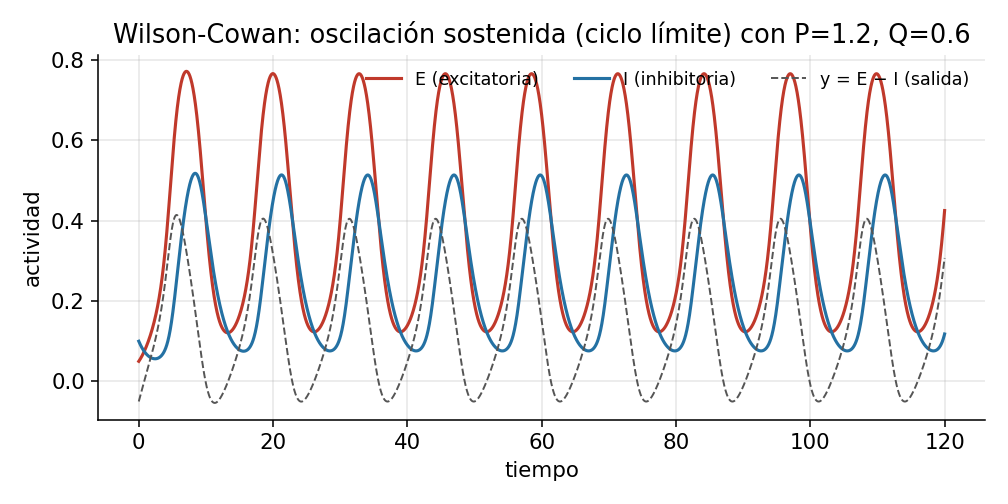
\includegraphics[width=0.85\linewidth]{fig_wc_series.png}
\caption{Series temporales de $I(t)$, $E(t)$ y la salida $y=E-I$ con los pesos por defecto y estímulos que llevan al régimen oscilatorio ($P\approx1.2$, $Q\approx0.6$). Tras un transitorio inicial, las poblaciones se estabilizan en una oscilación sostenida: el sistema cayó en un ciclo límite. (figura del proyecto)}
\label{fig:series}
\end{figure}

\subsection{Nulclinas, punto fijo y ciclo límite}
Formalmente (ver M2), analizamos el sistema en el plano de fases $(E,I)$. Las \textbf{nulclinas} son las curvas donde $\dot E=0$ y $\dot I=0$; su intersección es un \textbf{punto fijo} (equilibrio). Lo que caracteriza al régimen oscilatorio es que ese punto fijo es \textbf{inestable} --- un foco repulsor --- y está \emph{rodeado} por un \textbf{ciclo límite} estable. Las trayectorias que arrancan cerca del punto fijo espiralan hacia afuera; las que arrancan lejos, hacia adentro; todas terminan sobre la misma órbita cerrada. Esa órbita es la oscilación que vemos en las series temporales.

\begin{figure}[H]\centering
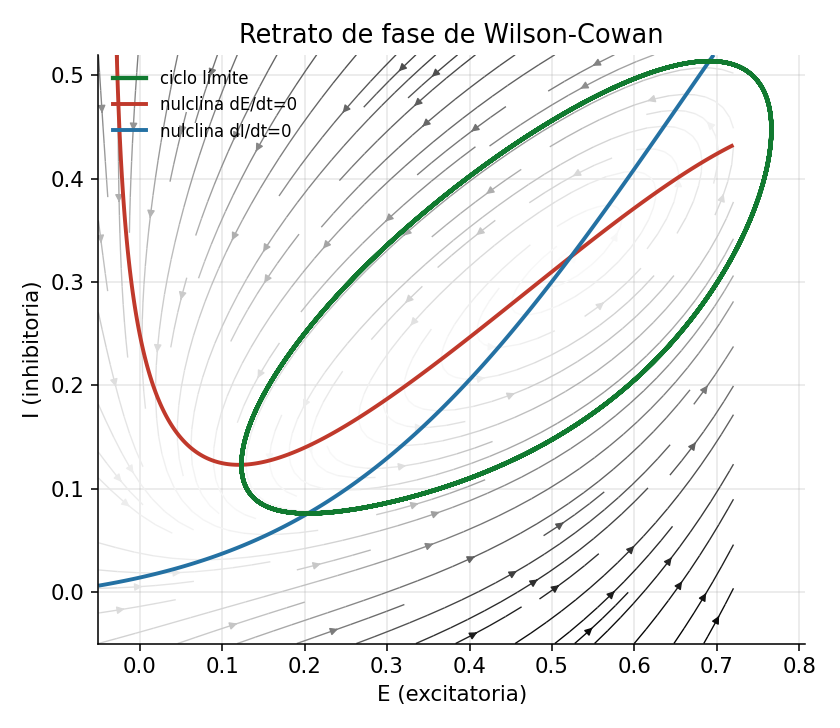
\includegraphics[width=0.75\linewidth]{fig_retrato_fase_wc.png}
\caption{Retrato de fase de Wilson--Cowan en el plano $(E,I)$: el campo vectorial, las dos nulclinas, el punto fijo inestable en su intersección y el ciclo límite estable que lo rodea. Las trayectorias, vengan de adentro o de afuera, convergen a la misma órbita cerrada. (figura del proyecto)}
\label{fig:fase}
\end{figure}

\subsection{Bifurcación de Hopf}
¿Cómo aparece o desaparece el ciclo? Vía una \textbf{bifurcación de Hopf} (ver M2 para el detalle): al variar un parámetro o el estímulo, el punto fijo pasa de estable a inestable cuando un par de autovalores complejos conjugados del Jacobiano cruza el eje imaginario. Justo en ese cruce nace (o muere) un ciclo límite de amplitud pequeña que luego crece. En términos prácticos: hay una \emph{frontera} en el espacio de estímulos que separa ``sistema quieto en un equilibrio'' de ``sistema oscilando''.

\begin{remark}[Dato concreto del proyecto]
Con los pesos por defecto de la Tabla~\ref{tab:params}, el sistema \textbf{oscila} (cae en el ciclo límite) para estímulos como $P\approx1.2$, $Q\approx0.6$. Pero \emph{no} basta con estar cerca: con $P=0.8$, $Q=0.6$ el mismo sistema cae en un \textbf{foco estable} (espirala hacia el equilibrio y se queda quieto), \emph{no} oscila. Es decir, cruzamos la bifurcación de Hopf al mover $P$. Conviene no confundir los dos regímenes: la misma máquina, con los mismos diez parámetros, hace cosas cualitativamente distintas según el estímulo.
\end{remark}

\section{Parámetros por defecto: por qué esos valores}

Los valores de la Tabla~\ref{tab:params} no son inventados: son \textbf{exactamente} los del simulador de MATLAB original del proyecto (\texttt{documentos/simulador\_wilson\_cowan.m}), y la implementación en Python (\texttt{src/wilson\_cowan/model.py}) es una traducción fiel. La razón de fijarlos así es doble:
\begin{enumerate}[nosep]
    \item \textbf{Reproducibilidad}: el ``sistema real'' que genera los datos sintéticos tiene que ser idéntico entre MATLAB y Python, para que los resultados de identificación sean comparables y auditables. El código incluso replica las tolerancias del integrador ($\texttt{rtol}=10^{-3}$, $\texttt{atol}=10^{-6}$) y usa RK45 ($\approx$ \texttt{ode45}).
    \item \textbf{Régimen adecuado}: estos valores están elegidos para que, con un estímulo razonable, el sistema \emph{oscile} (ciclo límite). Un modelo que solo relaja a un equilibrio sería un caso de identificación trivial y poco interesante; el régimen oscilatorio es donde la no linealidad importa y donde la identificabilidad se vuelve un problema real (por ejemplo, donde $w_{II}$ se esconde).
\end{enumerate}
Las condiciones iniciales por defecto son $E_0=I_0=0$ (reposo), y la simulación de referencia corre de $t=0$ a $600$ con \texttt{box\_pulse}$(0.8,100,400)$ en $P$ y \texttt{box\_pulse}$(0.6,200,500)$ en $Q$.

\section{Relación con ritmos cerebrales y variantes}

\subsection{Ritmos: gamma y theta}
El interés biológico de que Wilson--Cowan oscile es que la corteza \emph{está} llena de oscilaciones: ritmos que se miden en el EEG y que se asocian a funciones cognitivas. Dos son centrales para el proyecto:
\begin{itemize}[nosep]
    \item \textbf{Gamma} ($\sim$30--80 Hz): oscilación rápida generada precisamente por el lazo E/I local. El mecanismo E$\to$I$\to$E de la §5 es el modelo canónico de gamma (PING, \emph{pyramidal-interneuron network gamma}).
    \item \textbf{Theta} ($\sim$4--8 Hz): oscilación lenta que modula la amplitud de las ráfagas gamma. El código de un fenómeno cognitivo es el \textbf{acople theta-gamma}: ráfagas gamma ``montadas'' sobre la fase de theta.
\end{itemize}
El régimen objetivo del proyecto es justamente \textbf{theta-gamma}, y el generador \texttt{theta\_gamma\_pulse} lo induce: un tren gamma cuya amplitud modula una envolvente theta. B4 desarrolla esta conexión con ritmos y el rol del controlador en inducirlos.

\begin{remark}
Un detalle de unidades importante (documentado en el código): las frecuencias de los estímulos van en las mismas unidades de tiempo que la simulación, \emph{no} en los Hz biológicos. A $40$~Hz reales, con $\tau_e=1$, el sistema ni respondería. Lo que se conserva es la \emph{relación} gamma:theta $\approx 6{:}1$ y que caigan en la banda donde el sistema reacciona ($\approx 0.005$--$0.05$ en estas unidades).
\end{remark}

\subsection{Variantes del modelo}
El Wilson--Cowan que usamos es la versión ``de punto'' (una sola columna, sin extensión espacial). Hay dos extensiones estándar que conviene conocer:
\begin{itemize}[nosep]
    \item \textbf{Wilson \& Cowan (1973)}: los mismos autores extendieron el modelo a un \textbf{campo neuronal} (\emph{neural field}), donde $E$ e $I$ dependen de la posición espacial $x$ además del tiempo, y los pesos se vuelven \emph{núcleos} de conectividad $w(x,x')$ que decaen con la distancia. Esto permite modelar ondas viajeras y patrones espaciales, no solo oscilaciones temporales.
    \item Modelos de masa neuronal posteriores (Jansen--Rit, Deco et al.) que agregan más poblaciones o retardos, pero conservan la lógica E/I de Wilson--Cowan.
\end{itemize}
Para el proyecto nos quedamos con la versión de punto: es suficiente para tener oscilaciones no triviales, y mantiene el número de parámetros en diez, que es lo que queremos identificar.

\begin{thebibliography}{9}
\bibitem{wc1972} H. R. Wilson and J. D. Cowan, ``Excitatory and inhibitory interactions in localized populations of model neurons'', \emph{Biophysical Journal} 12(1):1--24, 1972.
\bibitem{wc1973} H. R. Wilson and J. D. Cowan, ``A mathematical theory of the functional dynamics of cortical and thalamic nervous tissue'', \emph{Kybernetik} 13:55--80, 1973.
\bibitem{ermentrout} G. B. Ermentrout and D. H. Terman, \emph{Mathematical Foundations of Neuroscience}, Springer, 2010.
\bibitem{izhikevich} E. M. Izhikevich, \emph{Dynamical Systems in Neuroscience}, MIT Press, 2007.
\end{thebibliography}

\end{document}
